\subsection{Related Standards}
\subsubsection{C++14} C++ will be programmed according to the C++14 standard provided by Texas Instruments' ARM compiler. This standard is formally known as
\href{https://www.iso.org/standard/64029.html}{ISO/IEC 14882:2014}. C++ is
a superset of C, and builds upon it by introducing object-oriented
programming concepts while maintaining the functional language aspect of C.

\subsubsection{802.11} The microcontroller (MCU) supports transmission through the Institute of
Electrical and Electronics Engineers (IEEE) 802.11b/g/n standard of wireless
communication. This standard uses the S band of radio frequences and
operates at 2.4 GHz. There are 14 accessible channels, each spanning a band
width of 22 MHz (pictured in \autoref{wifi_channels}).
\begin{figure}[H]
    \caption{802.11b/g/n channels \cite{Flickenger}}
    \label{wifi_channels}
    \centering
    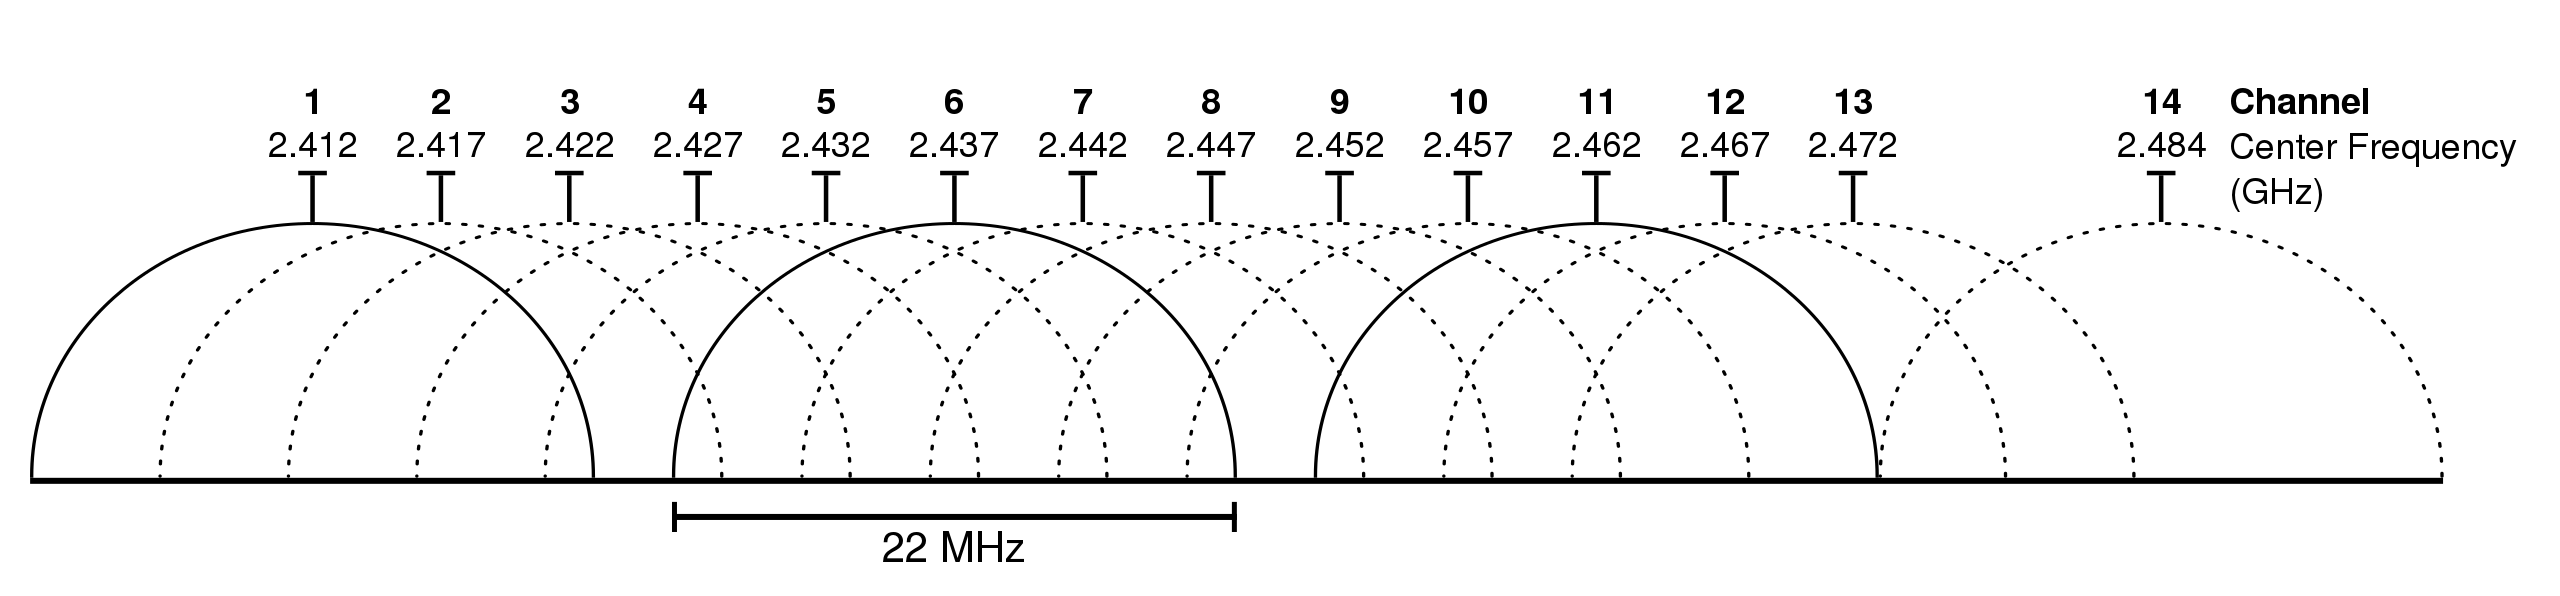
\includegraphics[width=\textwidth]{images/wifi_channels.png}
\end{figure}
These channels specifically reside in an industrial, scientific and medical
(ISM) band. This standard also provides datagram frames for the transport
layer.

\subsubsection{TCP} \label{tcp_standard} Transmission Control Protocol (TCP) will be used to satisfy transport layer
requirements of the product, and will be used to transmit symbols (i.e.
from any commands, data, settings, telemetry, etc.) between Amazon Web
Services (AWS) and the microcontroller (MCU). TCP was chosen over other
protocols, such as User Datagram Protocol (UDP), mainly due to its
reliability. The extent of TCP's reliability includes features such as
checksums, duplicate data detection, retrying of transmissions, sequencing,
and timers.
Such reliability is favored over higher bandwidth or lower
latency, as neither of the latter are required for the kilobytes
of information being relayed between AWS and the MCU. A standard TCP frame
is shown in \autoref{tcp_frame}.
\begin{figure}[H]
    \caption{TCP frame \cite{Kristoff}}
    \label{tcp_frame}
    \centering
    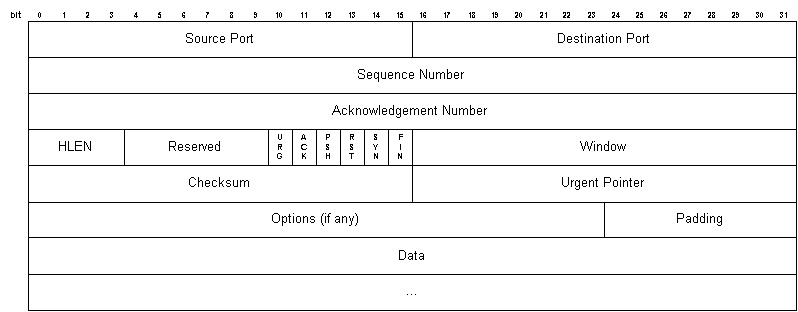
\includegraphics[width=\textwidth]{images/tcp_frame.jpg}
\end{figure}


\subsubsection{IPv4} IPv4 is the fourth version of the Internet Protocol, a network layer protocol in use to relay data between devices and across networks. The data relayed, datagrams, are sent between sources and hosts that are identified by 32-bit addresses. This protocol strictly functions to transport the datagram from one device to another, with no end-to-end reliability, flow control, sequencing, or other measures found in other protocols such as TCP. IPv4 provides two distinct features: fragmentation of whole datagrams, and addressing of devices. A standard IPv4 frame is shown in \autoref{ipv4_frame}.
\begin{figure}[H]
    \caption{IPv4 frame \cite{Postel1981}}
    \label{ipv4_frame}
    \centering
    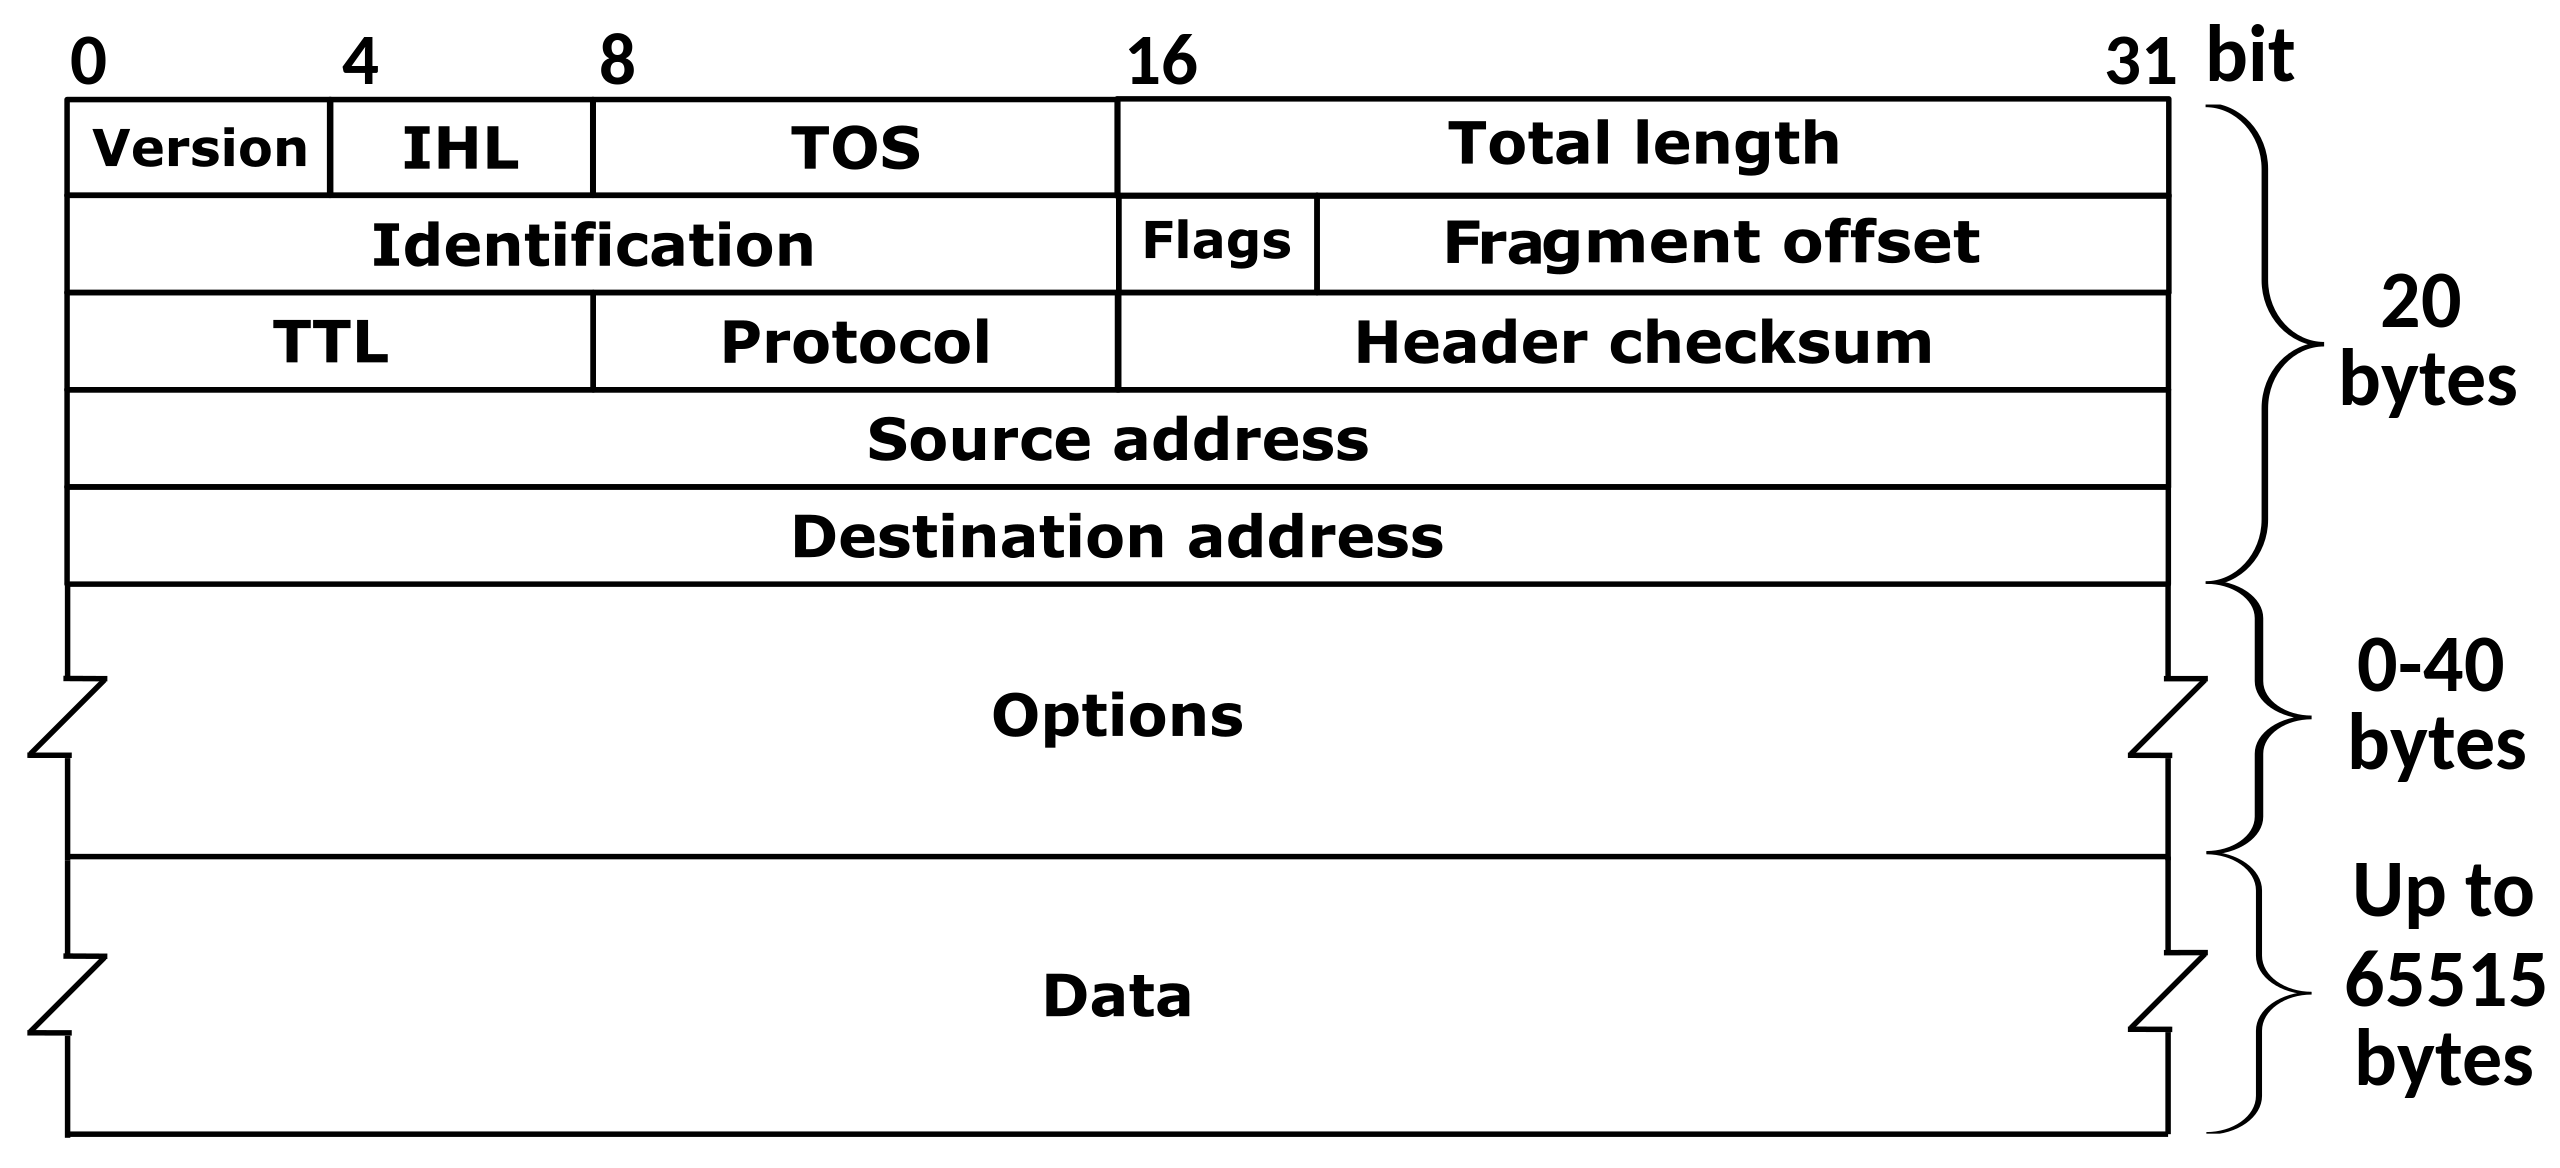
\includegraphics[width=\textwidth]{images/ipv4_frame.png}
\end{figure}